\section{Derivation of the affects of angles on the imaging plane}
Some of this document needs updating.\footnote{Equation indices not updated!! Should fix this later, as numbering will be off.}

\subsection{Analyzing an adjustment of SM2}
In general, the principle being applied here is that the angle of incidence is equivalent to the angle of reflection. In other words, the light ray's incoming angle relative to the plane of the mirror is equivalent to its outgoing angle.\\
For a mirror aligned to keep the beam travelling relative to the optical plane, an adjustment of $\theta_{mechanical}$ will lead to an adjustment of $\theta_{optical} = 2\theta_{mechanical}$ from the optical axis. In this document, we will be referring specifically to the optical quantities. \\
We begin with the Hestia system, which includes two mirrors, Steering Mirror 1 (SM1) and Steering Mirror 2 (SM2). We know the use of these mirrors enables the control of the light sheet in the imaging plane. The diagram below illustrates the placement of SM1 and SM2 as well as their positioning relative to the optics of interest.\\
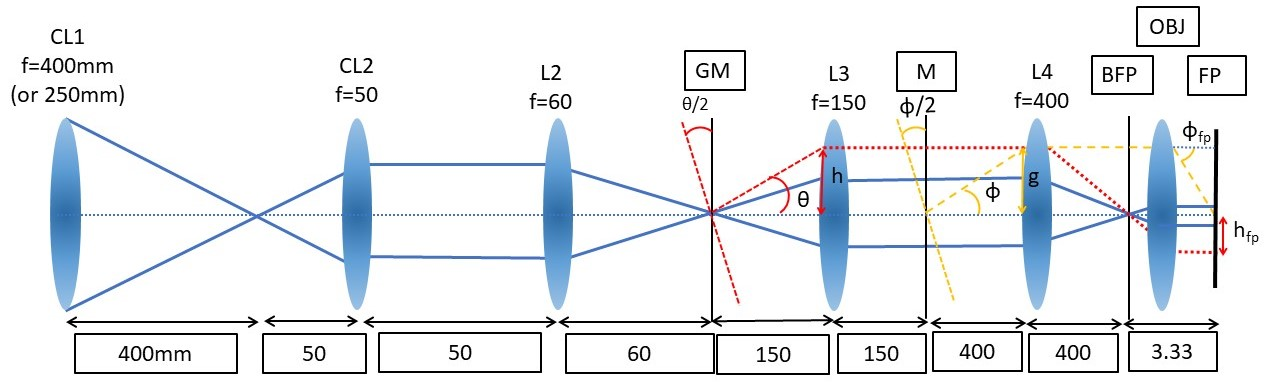
\includegraphics[width=\textwidth]{Hestia_HIST_Computation_Fig1}
\begin{center}
    Impact of an SM2 Adjustment
\end{center}
From the figure above, it is clear that $\phi$ is an angle within a right triangle with width 125mm and an unknown height. We immediately see that the height $h$ is given by
\begin{gather}
    \tan(\phi)=\frac{125mm}{h_2}\\
    g = 125mm \tan(\phi)
\end{gather}
The McLauren series of $\tan(\phi)$ is given by:
\begin{gather}
    \tan(\phi) = x+\frac{x^3}{3} + \frac{2x^5}{15} + ...\\
    \text{for   } \phi<<1, \ \tan(\phi) \approx x
\end{gather}
Therefore, in millimeters, $h = 125\phi$.
Following the diagram, we see that after 125mm our ray is collimated by another 125mm lens, and then proceeds 250mm until it impacts yet another 125mm lens. Since our ray started on the optical axis and got to $g$ over the course of 125mm, we know it will be focused back down to the optical axis in the same distance with the same angle $\phi$. The ray then continues from this intersection for another 200mm with the same angle $\phi$, reaching a  (negative by convention) position relative to the optical axis of:
\begin{gather}
    g_{bfp} = -200mm*\tan(\phi)\\
    g_{bfp} \approx -200mm \phi
\end{gather}
$h_2$ is the angle with which the beam enters the objective. The objective focuses the ray back to the optical axis in the sample over a distance which may be determined by its magnification rating as follows:
\begin{gather}
    \frac{f_{TL}}{magnification} = f_{obj}
\end{gather}
Taking an example of a 40x magnification with a 200mm tube lens (which is what we have in our system)
we see that for an angle of incidence in the sample $\alpha$, we traverse the displacement $g_{bfp}$ in $f_{obj}$. We drop the negative on the height, but note that the ray is coming from the "bottom" side of the objective, meaning it has crossed over the optical axis and is on the opposite side from where it originated. All this considered, we see that:
\begin{equation}
    \tan(\phi_{fp})= g_{bfp}/f_{obj}
\end{equation}
substituting for $g_{bfp}$ in the small angle approximation from the previous equation, we see that
\begin{equation}
    \tan(\phi_{fp}) = \frac{200mm \times \phi}{f_{obj}}
\end{equation}
so that more generally
\begin{gather}
    \tan(\phi_{fp}) \approx \frac{f_{TL}}{f_{obj}} * \phi\\
    \tan(\phi_{fp}) \approx M*\phi\\
    \phi_{fp} \approx \arctan(\frac{f_{TL}}{f_{obj}} * \phi)
\end{gather}
Note that this angle in the imaging plane is likely to be quite large, since the slope of the ray has been increased by a factor of 60. As a result, we can no longer reasonably use the small angle approximation.
Alternatively, for a $\theta$-objective, which is designed to follow the small angle approximation even for large $\theta$ and is widely used in certain applications due to the computational simplicity such a relation entails, we see that
\begin{equation}
    \phi_{fp} = \frac{f_{TL}}{f_{obj}} * \phi
\end{equation}
So now we see the relationship between the angle in the conjugate steering mirror plane and the angle in the sample plane.

\\
\begin{center}
    Impact of an SM1 Adjustment
\end{center}
Let the optical adjustment of SM1 be denoted as $\theta$. A ray affected by this mirror rotation is given by \begin{gather}
    \tan(\theta)= \frac{h}{125mm}\\
    \theta = \frac{h}{125mm}\\
    h= {125mm}*\theta
\end{gather}
where we are again making use of the small angle approximation. We now see from the optical diagram that this height is conserved as it moves down the optical train. It flips over the optical axis but its distance is conserved until it reaches the tube lens. Upon reaching the tube lens, it descends to the optical axis over a span of 200mm. As a result, it forms a new angle $\theta_{bfp}$ at the back focal plane relative to the optical axis. We therefore see that
\begin{gather}
    \theta_{bfp} = \frac{125mm*\theta}{200mm}
\end{gather}
Where since this angle is small we again make use of the small angle approximation. Approximating the objective as a simple lens, we see that the position of the light sheet in the sample plane is given by:
\begin{gather}
    x_{sp} \approx f_{obj} \frac{125\ \theta}{200}
\end{gather}
Recall from before that incident angle is given by:
\begin{gather}
    \phi_{fp} = \arctan(\frac{f_{TL}}{f_{obj}}\phi)\\
    \phi_{fp} = \arctan(\phi * magnification)
\end{gather}
\newpage
\begin{center}
    \textbf{Analysis of the HIST Optical System } 
\end{center}
Now we follow the same line of reasoning for the HIST setup as specified in Tang et al. (2018), again analytically tracing the pathway of a ray affected by rotations of the galvomirror GM and control mirror M. Note from the figures that the galvomirror and the control mirror are both near to the tube lens in the optical train, so this calculation is slightly simpler. See the figure below for a diagram of the relevant optical components.
\begin{center}
    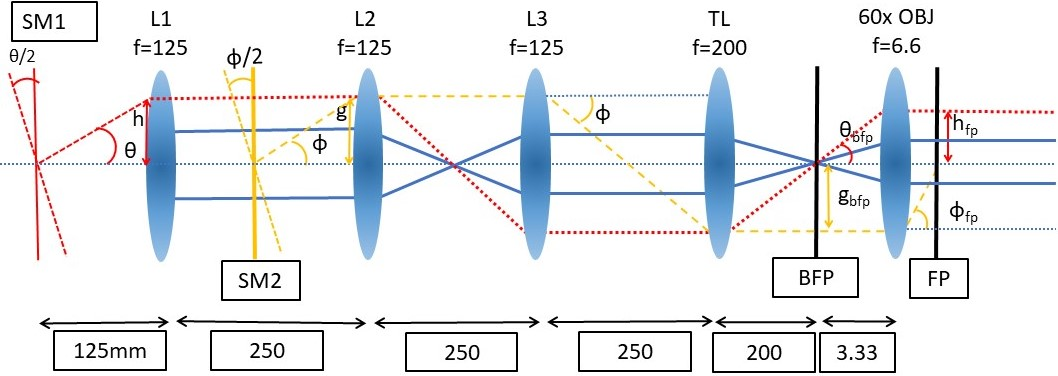
\includegraphics[width=\textwidth]{Hestia_HIST_Computation_Fig2.jpg}
\end{center}
The displacement at the tube lens as a result of the adjustment of the control mirror by an optical angle $\phi$ is given by
\begin{gather}
    \frac{g}{d} = \tan(\phi) \approx \phi.\\
    \phi*d \approx g
\end{gather}
Here we can see that the distance between SM2 and L2 is 125mm, so $d=125mm$. We note that the displacement at the tube lens, however, is given by
\begin{gather}
    \phi = g_{bfp}/f_{TL}\\
    g_{bfp} = \phi f_{TL}
\end{gather}
since the ray passes through the optical axis one tube-lens focal length prior to the tube-lens with an angle of $\phi$ relative to the optical axis. As before, we then compute the angle of incidence in the focal plane to be
\begin{gather}
    \tan(\phi_{fp}) = \frac{g_{bfp}}{f_{obj}}\\
    \tan(\phi_{fp}) = \phi \frac{f_{TL}}{f_{obj}}\\
    \phi_{fp} = \arctan(\phi \frac{f_{TL}} {f_{obj}})\\
    \phi_{fp} = \arctan(\phi * magnification)
\end{gather}
where $\phi_{fp}$ is again too large to use the small angle approximation.
This displacement changes the angle going into the back focal plane, which in turn influences the angle coming out of the back focal plane, and therefore the placement of the beam in the sample. The exact distance 
The galvomirror, similarly to SM2, produces an adjustment of the ray's distance from the optical axis going into the tube lens, essentially adding an "offset" to the beam. This offset for small theta is given by
\begin{gather}
    \frac{h}{150mm}=\theta\\
    h=150mm \ \theta
\end{gather}
In the back focal plane of the objective, this corresponds to a change in angle given for small angles by
\begin{gather}
    \theta_{bfp} = h/400mm
\end{gather} 
so therefore in the sampling plane it is again a change in position given by
\begin{gather}
    h_{fp} = 3.33mm*\theta_{bfp}
\end{gather}
where we again use the small angle approximation to simplify the expression.
Thus the galvomirror does in fact change position, as we had thought. The authors note and explain this in their methodology section, so it would appear that their figure, which appears to show the galvomirror's rotation causing a change in angle of the lightsheet and contributing to a windshield-wiper motion in the imaging plane. This is actually the function of the mirror, which determines the angle of the lightsheet and seems to be manually adjusted when necessary in-between experiments.
\newpage
\begin{center}
    \textbf{Microscope Resolution and Camera Pixel Size}\\
\end{center}
The Raleigh Criterion relates the diffraction-limited angle of minimum resolution, i.e. the smallest angle at which an objective can tell two objects apart, to the wavelength $\lambda$ and lens aperture $D$. This relationship may be formulated as
\begin{gather}
    \sin(\theta_{min}) = \frac{1.22\lambda}{\mathcal{D}}.
\end{gather}
Since $\theta_{min}$ is a very small angle, we use the small angle approximation, simplifying the expression to
\begin{gather}
    \theta_{min} = \frac{1.22\lambda}{\mathcal{D}}.
\end{gather}
Trigonometrically, we can relate $\tan(\theta_{min})$ to the ratio of the smallest distance between two differentiable points $\Delta l$ and the distance to the subject. In a microscope which is in focus, the distance between the objective and the subject is approximately equal to the focal length of the microscope $f$. This leaves us with the expression:
\begin{gather}
   \frac{ \Delta \mathcal{L}}{f}= \tan(\theta_{min})
\end{gather}
Multiplying by the focal length, using the small angle approximation and substituting for $\theta_{min}$ leaves
\begin{gather}
    \Delta \mathcal{L} = \frac{1.22f\lambda}{\mathcal{D}}.
\end{gather}
Alternatively, Murphy (\textit{Fundamentals of Light Microscopy and Electrical Imaging}, p.87) formulates the diffraction resolution limit for specifically fluorescent systems as a more generous
\begin{gather}
    \Delta \mathcal{L}=\frac{0.61\lambda}{NA}.
\end{gather}
Since the light's path to the CCD is through the same objective it just traversed, it is magnified so that the distance between two such minimally differentiable points on the image at the camera's CCD is clearly given by 
\begin{gather}
    \Delta \mathcal{L}_{CCD} = \mathcal{M} \Delta \mathcal{L}
\end{gather}
where $\mathcal{M}=\frac{f_{TL}}{f_{obj}}$ is the magnification power of the microscope. As such, we see that increasing the magnification of the microscope also increases the size of the smallest detectable detail on the CCD. It is important to balance the resolution with the magnification to ensure one is capturing enough information to accurately reconstruct a digital image without oversampling and saving lots of useless information.
The Nyquist Conditions determine the sampling rate required for accurate digitization of analog data without loosing information. A minimum of two pixels per minimum resolvable distance is required, but most sources agree that around 2.5-3 is a better ratio for microscopy.
Let $\mathcal{N}$ be the number of pixels per smallest resolvable feature. Then we see that optimal pixel size $\mathcal{S}$ is given by
\begin{gather}
    \mathcal{S} = \frac{\Delta \mathcal{L}_{CCD}}{\mathcal{N}}\\
    \mathcal{S} = \frac{\mathcal{M} 1.22f\lambda}{\mathcal{D}\mathcal{N}}
\end{gather}
\begin{center}
        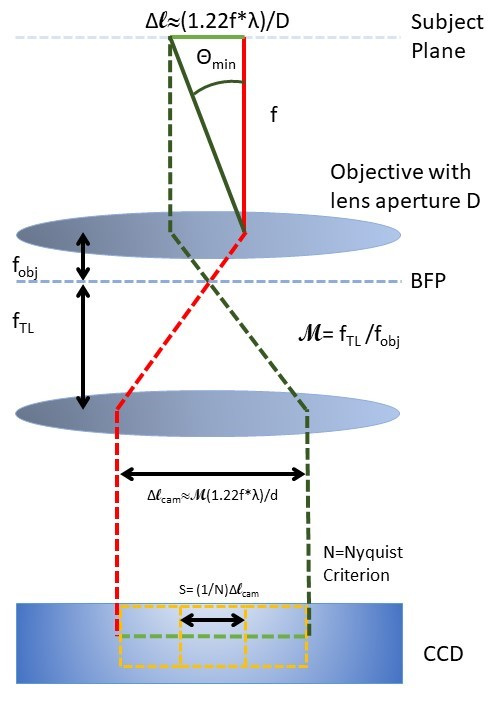
\includegraphics[scale=.7]{Nyquist_Pixel_size.jpg}
\end{center}

\newpage
\begin{center}
    \textbf{Further Calculations on Displacement of Lightsheet}
\end{center}
Based upon the reference sheets for the the steering mirrors, we know that the mirrors work linearly (?) on a scale of 0-10 Volts, resulting in an adjustment of up to 1.5 degrees at the maximum of 10V. Therefore, the range of angles for $\theta_{mechanical}$ and $\phi_{mechanical}$ is 0-1.5 degrees, while the corresponding maximum optical angles are 0-3 degrees for each.
The maximum displacement in the imaging plane is when $\theta_{mechanical}=1.5 \ degrees \ \therefore \ \ \theta = \frac{3\pi}{180}$,
which gives
\begin{gather}
    x_{sp \ max} = 3.33mm * \frac{125mm}{200mm}*\frac{3\pi}{180} = 108.3\mu m
\end{gather}
Similarly, from (19) we see that the the maximum incident angle in the imaging plane is:
\begin{gather}
    \phi_{sp \ max} = \arctan(\frac{f_{TL}}{f_{obj}}*\frac{3\pi}{180})
\end{gather}
For a 60x objective, this yeilds:
\begin{gather}
    \phi_{sp \ max} = \arctan(\pi) = 1.2626 \ radians
\end{gather}
Or, in the case of a theta lens:
\begin{gather}
    \phi_{sp \ max} = (f_{TL}f_{obj}*\frac{3\pi}{180}) = \pi \ radians 
\end{gather}
The theta lens approximation seems impractical as it would have to be acting as a mirror to reflect the ray back in the direction it came. This seems unlikely to be physically accurate.\\

We now will look into the Gaussian optics, including the beam width and other parameters of the laser system.
The Rayleigh length is defined to be "the distance along the propagation direction of a beam from the waist to the place where the area of the cross section is doubled." (Source: Wiki.) In simpler terms, this value gives the distance from the narrowest point of a focused beam to the point where, in either direction, its width has doubled.
\begin{gather}
    z_r = \frac{\pi \omega_0^2}{\lambda}
\end{gather}
It is also possible to check the beam width at any given distance $d$ from the beam width via the following function:
\begin{gather}
    w(z) = w_0\sqrt{1+\frac{z}{z_R}}
\end{gather}
Now we must determine the relationship between the beam waist formula and its relationship to beam size in the back aperture. The Diameter of a beam waist is inversely proportional to the angular spread of the beam's divergence from the focal point, where divergence is defined as the angle at which a ray converges to the geometric focal point $\Theta_{div}$.This relationship is given as follows:
\begin{gather}
    \omega_0 \approx \frac{2 \lambda }{\pi \Theta_{div}}
\end{gather}
Since lenses with smaller focal-length-to-incoming-beam-size ratio have a larger angular approach to the geometric focal plane, we see that increasing the incoming beam size for a given lens also increases $\Theta_{div}$, and therefore causes a decrease in the beam waist width. This essentially means that the thinness of our beam waist is effectively limited by the size of the back aperture on our objective, which limits the maximum beam size in the back focal plane which our setup can accommodate. More formally, we know that for an objective with a back aperture 
\begin{gather}
    f_{back} \geq 2*g_{bfp}
\end{gather}
Where $g_{bfp}$ is the beam radius at the back aperture introduced by the rotation of SM2, as defined in equation (24).
That being said, getting the beam width too large in the back focal plane also runs up against the limits on incident angle caused by the Numerical Aperture as well as the practical limits caused by the finite size of the back aperture. Numerical aperture is given by:
\begin{gather}
    NA = nsin\phi_{NA \ max}\\
    \arcsin(\frac{NA}{n}) = \phi_{NA \ max}    
\end{gather}
Thus, if the ray is going into an object with a high index of refraction, the maximum allowable angle may be relatively small, putting a significant cap on the beam size, especially in the context of a HIST based system, which already requires a certain amount of beam offset to create the highly inclined tile.
Essentially, the issue here is thus that we have the requirement that
\begin{gather}
    \phi_{NA \ max} \geq \phi_{bfp}\\
    \arcsin(\frac{NA}{n}) \geq \phi_{bfp}
\end{gather}
meaning that farthest point of the HIST beam given by the sum of the displacement in the back focal plane induced by SM2's rotation and the radius of the illumination beam on any given axis cannot be located so far away that the ray approaching the focal plane exceeds the maximum angle allowed by the NA in a given medium. In other words:
\begin{gather}
    \arctan(\frac{g_{bfp} + r_{beam}}{f_{obj}}) \leq \phi_{bfp \ max}\\
    \arcsin(\frac{NA}{n}) \geq \arctan(\frac{g_{bfp} + r_{beam}}{f_{obj}})
\end{gather}
Recalling our earlier investigation into Microscope Resolution gives that for fluorescent microscopy, it is clear that while a larger NA value enables a larger beam in the back focal plane and thus a greater HIST incident angle, it also increases the diffraction-limited resolving power the microscope can provide.\\
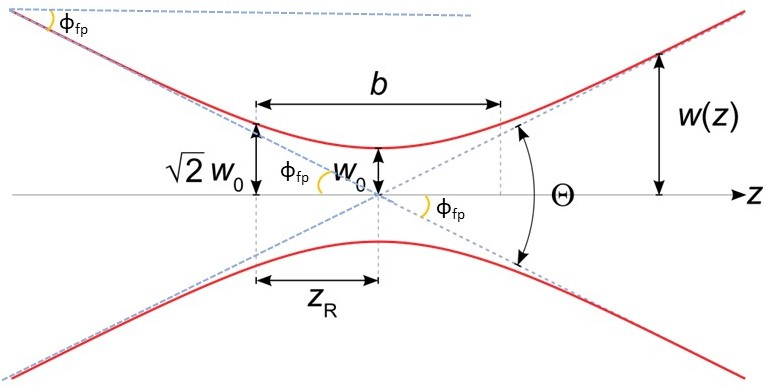
\includegraphics[width=\textwidth]{Hestia_HIST_Computation_Fig3.jpg}\\
Image adapted from Wikipedia.
\newpage
\begin{center}
    \textbf{Determining optimal NA size}
\end{center}
Ideally, in order to maximize the microscope's resolving power and minimize $\Delta \mathcal{L}$, we must determine the maximum $\phi_{fp-max}$ given by the scenario in which the maximum incoming beam width the back focal plane can accommodate is used, so $f/=g_{bfp}$. This will in turn grant the narrowest beam due to the largest $\Theta_{div}$ being as large as the back aperture can accommodate. However, we also notice that the there is a limit imposed on the front of the objective by the Numerical Aperture, as given in equation (50). As such, this also places a limit on $\Theta_{div}$, so that either the numerical aperture or the back aperture will place a limit on the size of $\theta_{fp}$. Note that larger back focal plane means greater magnification $\mathcal{M}$, as does a larger $\phi_{NA max}$, so both of these limitations are really noting that magnification and beam-fineness is increased by NA while the minimal resolution length $\mathcal{L}$ is decreased by NA. As such, one must find the necessary balance between magnification and resolution for a given sample.\\
FIND EXPRESSION RELATING MAGINIFICATION TO RESOLTUION OR AT LEAST CONSTRUCT A TABLE!! Should relate L and M.
\begin{gather}
    \mathcal{L} = \frac{0.61\lambda }{nsin\phi_{NA \ max}}
\end{gather}
Let us assume the back aperture is at least large enough to accommodate a beam diameter sufficient to induce $\phi_{NA \max}$. Then we see that $\phi_{fp} = \phi_{NA \ max}$, so this should somehow induce some sort of magnfication limit--not sure exactly what yet. 
That being said, here is a table of values from microscopy-u detailing NA and magnification relations.\\
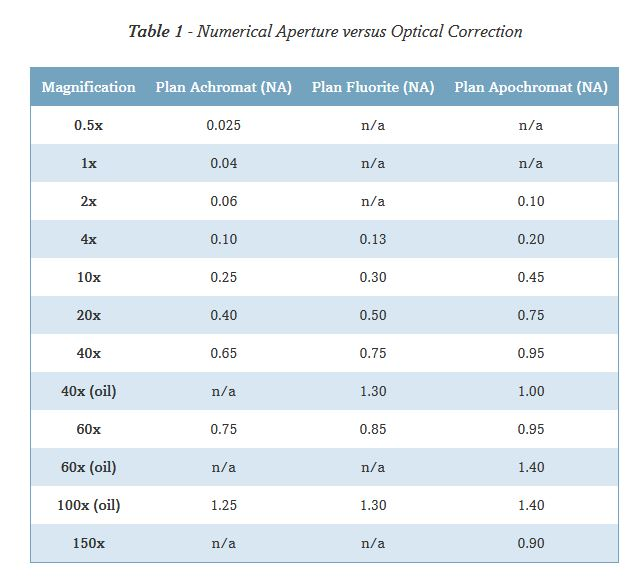
\includegraphics[width=\textwidth]{num_aperture_magnification_table.JPG}
\newpage
\newpage
\begin{center}
    \textbf{Temporal and physical Limitations of Hestia's HIST}
\end{center}
See Hestia Components and Limitations in Teams for full analysis. Should summarize here at some point.
The takeaway so far is that we are limited in between frames by steering mirrors for ROIs less than half of the CCD (which limits us to 5ms/frame or higher), since they take 5ms or less. Actual minimum adjustment time is unavailabe from the manufacturers and would require precise \textit{in situ} testing via potentiometers.
In between focal planes, we must wait for the Optotune lenses to adjust to the new focal plane. According to optotune, this will take 5ms to move and 25ms to settle, which is longer than the typical $\leq 5$ms one millirad mirror step. That being said, it is not  clear how long larger mirror steps will take, so the mirror spooling across a "large" number of radians to reset to a starting position for the next focal plane may take longer than the optotune. Note that waiting for settling may not be necessary, especially if there are a lot of images per focal frame so that being slightly out of focus for the first few mirror steps of a plane while the optotune settles isn't such a big deal. That being said, this may also provoke a consistenly blurred image in certain sectors of the imaging plane, so that the same parts of each slice are poorly resolved. It may also be possible to offset the mirror by a certain amount so that the first image or two are still collected off of the immediate region of interest, so that the blurred area is not in the area where the subject is anticipated, i.e. we essentially delay by gathering a couple extra lower quality frames rather than just idling the system.\\
Whichever SM controls the non-interating placement of the lightsheet (lets call this the vertical placement for consistency). If the Steering Mirror takes a long time to spool across the entire field of view back to its starting point (i.e. significantly longer than the optotune's effective refocusing time) it may be advantageous to simply leave it in place and proceed from there in the next frame. In other words, we would do Level 1: Leftmost-to-Rightmost Level 2: Rightmost-to-Leftmost Level 3: Lefttmost-to-Rightmost etc. Is this doable with image processing software?\\
At some point, I ought to test the response times of the mirrors over a variety of ranges, from smallest possible steps to full range transversal.
\\
Limitations are given by the maximum and minimum value attainable by each component. For instance, the maximum values of each steering mirror is $\pm 1.5$ degrees, the maximum optotune values are -2 dioptic power to +3 dioptic power (assuming its the fast version.) I'm not yet certain how to determine how much this changes the focal plane placement of the object-unsure of how to compute this change. That being said, the maximum range depending on the mirrors can be easily found using the formulae derived previously in this document. See formulae 41-44, where we note that for a non-theta lens, a 60X objective yields a 1.2626 radian angle in the sampling plane and up to a 108.3$\mu m$ displacement.
The camera's maximum framerate for a vertical bin is given approximately as follows:
\begin{gather}
    max \ fps \approx 101 * (\frac{2048}{section\ width})
\end{gather}
A table is provided by Andor detailing more precise figures, since progressively more efficiency is lost as the section width decreases.
Note that most OBIS lasers are technically capable of 500kHz modulation rate via analog modulation and a higher rate via digital modulation, so unless there is an intervening hardware limitation I'm not aware of, the lasers are the fastest component by far and will never impose a timing bandwidth. In fact, if I understand correctly, most OBIS lasers switch on in a fraction of a microsecond, so it is very easy to synchronize the laser's activity with the CCD's active exposure period. This is good since it allows efficient light use, so that we may effectively and precisely restrict the time the laser spends on to the precise time it is needed, minimizing phototoxic affects on the subject.\\
That being said, the actual limit in this situation is the AOTF's abilities. I'm not sure where to find this information, but I'll dig it up. I know that the AOTF is known to have been run successfully in the past on a 5ms scheme, so it stands to reason that the AOTF is capable of something faster than that, which still leaves the steering mirrors as by far the largest delay in the proceedure.
Update this information. Note that the AOTF is massively fast, and is probably the fastest component we have.
\newpage
Note that we must also offset the planar motion of the intersection between the focal plane and the slanted lightsheet. Whatever our angle is, we must compute how much horizontal motion a given vertical increment causes and then offset the height in the focal plane by adjusting SM1 appropriately in the next sweep. For instance, if the angle of the light sheet is $\phi_{fp}$ degrees, then $h_{fp-offset}= \frac{y_offset}{\tan(\phi_{fp})}$, where $y_offset$ is the vertical offset from the initial focal plane. Doesn't really matter we start as long as we make this adjustment to keep things in line as the focal plane changes and the scan progresses.
\newpage
\textbf{Concerning ETLs--BAD, SLATED FOR DELETION}\\
    ETL 1 allows for rapid transitions between widefiedl and point illumination. Note SM1 is conjugate to the Back Focal Plane of the Objective and SM2 is optically conjugate to the sample plane, so that setting ETL1 $f=\infty$, then we will end up with a wide plane at the objective back focal plane and thus a diffraction-limited spot at the sample. Inversely, if we adjust ETL1 such that it focuses to a spot at SM1, the light will form a wide colimated beam at the sample. ViewMod states that in module 4:
"We use a 4f system to
relay the beam and position a second ETL (ETL2) (EL-16-40-TC, Optotune) midway
between the second and third relay lens (conjugate to the BFP of the objective). Adjusting the
focal length of ETL2 subsequently scans the focus of the illumination light axially." 
In module 5, we have ETL3 to change the focal point of the image without adjusting the objective, allowing us to decouple focusing excitation and the image in spite of the fact that they both move through the same objective. This should be a slight adjustment, as large changes will change the magnification of the image significantly.
\begin{center}
    \textbf{Use Cases}
    Finish me up tonight complete with illustrations.
\end{center}
\newpage
\begin{center}
    \textbf{Wiring and Coding Documentation as well as Use Cases/Necessary Additions\\ FIGURE OUT COM PORT ASSIGNS}
\end{center}
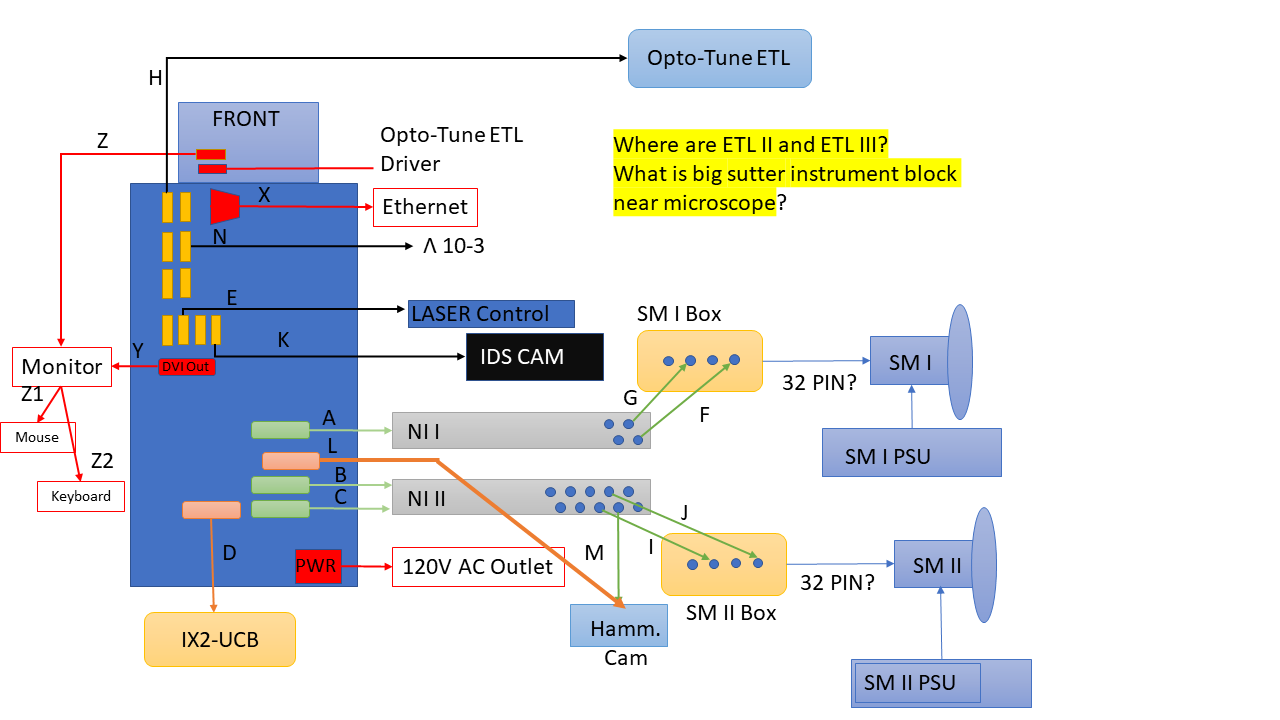
\includegraphics[width=\textwidth]{Hestia_wiring_img_1-9-23.png}


\newpage
\begin{center}
    Cumulative Circuit Diagram of HESTIA with all COM ports, Devices, etc. ONLY THING WE SHOULDN'T HAVE IS niDAQ-> SM boards->SMs
\end{center}

\newpage
\begin{center}
    \textbf{Computation of change in focal plane position in the sample caused by a known displacement in the objective medium}\\
\end{center}
\fbox{\begin{minipage}{\textwidth}
\textbf{Summary\\ A one unit translation of the objective will produce a translation of the focal plane $n_3/n_1$ units in the same direction, where $n_3$ is the index of refraction of the sample and $n_1$ is the index of refraction of the objective's immersion media.}
\end{minipage}}
In this computation, we are going to use the matrix method to find how much a displacement of the objective will move the focal plane in the sample. We assume an immersion media of known depth $D_1$ and homogeneous index of refraction $n_1$, a coverslip with index of refraction $n_2$ and depth $D_2$, and a sample of homogeneous index of refraction $n_3$ and depth $D_3$. Diagram included below for reference.
\begin{figure}[h]
    \centering
    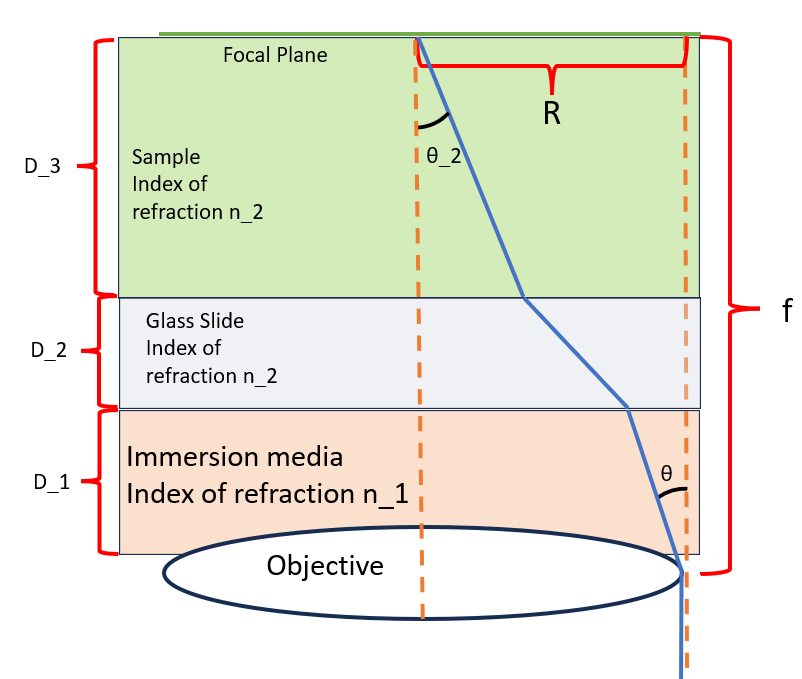
\includegraphics[width=0.7\linewidth]{image3.png}
    \caption{A diagram of the setup described below.}
    \label{fig:enter-label}
\end{figure}
\\Using matrix formalism, we find the expression:
\begin{gather}
    \begin{bmatrix}
        0 \\ \theta_2
    \end{bmatrix}
    = 
    \begin{bmatrix}
        1 & D_3\\ 0 & 1 
    \end{bmatrix}
    \begin{bmatrix}
        1 & 0\\ 0 & n_2/n_3 
    \end{bmatrix}
    \begin{bmatrix}
        1 & D_2\\ 0 & 1 
    \end{bmatrix}
    \begin{bmatrix}
        1 & 0\\ 0 & n_1/n_2 
    \end{bmatrix}
    \begin{bmatrix}
        1 & D_1\\ 0 & 1 
    \end{bmatrix}
    \begin{bmatrix}
        R \\ \theta
    \end{bmatrix}
\end{gather}
Explication from left to right:\\
\begin{itemize}
    \item leftmost matrix is the ray at the focal plane. In order to be focused, it must definitionally have a radius of 0. It will also have some angle $\theta_2$, which is determined purely by $\theta$ and the refraction of the beam at the junctions between media with different refractive media.
    \item Third distance transfer matrix, which represents the propogatinon of the ray through the sample some distance $D_3$ to the focal plane.
    \item Second refraction matrix. Accounts for the refraction of the beam between the coverslip and the sample.
    \item Second distance transfer matrix, which represents moving the ray propogating through the glass coverslip some fixed distance $D_2$.
    \item First transfer matrix. Represents the refraction of the rayat the boundary between the immersion media and the coverslip.
    \item First distance transfer matrix, which represents the propogation of the ray some distance through the immersion media.
    \item This matrix represents the incident ray exiting the objective lens, which is some distance R from the middle of the lightpath and has an orientation $\theta$. Note $\theta$ will be negative, meaning it slants downwards by some angle $\theta$, as given by the formula for the numerical aperture of the objective. Using the small angle approximation for sine, we see this can be given by $NA=n_1 \sin \theta \approx n_1 \theta$.
\end{itemize}
Note an implicit assumption of our model is that the focal plane lies within the sample; this model will not hold if the focal plane of the microscope ends up in the glass slide. 
\\We may rewrite this in terms of the focal length of the lens to get the equation in terms of $R$ alone, eliminating the variable of $\theta$. See figure 2 below for reference.
\begin{figure}[h]
    \centering
    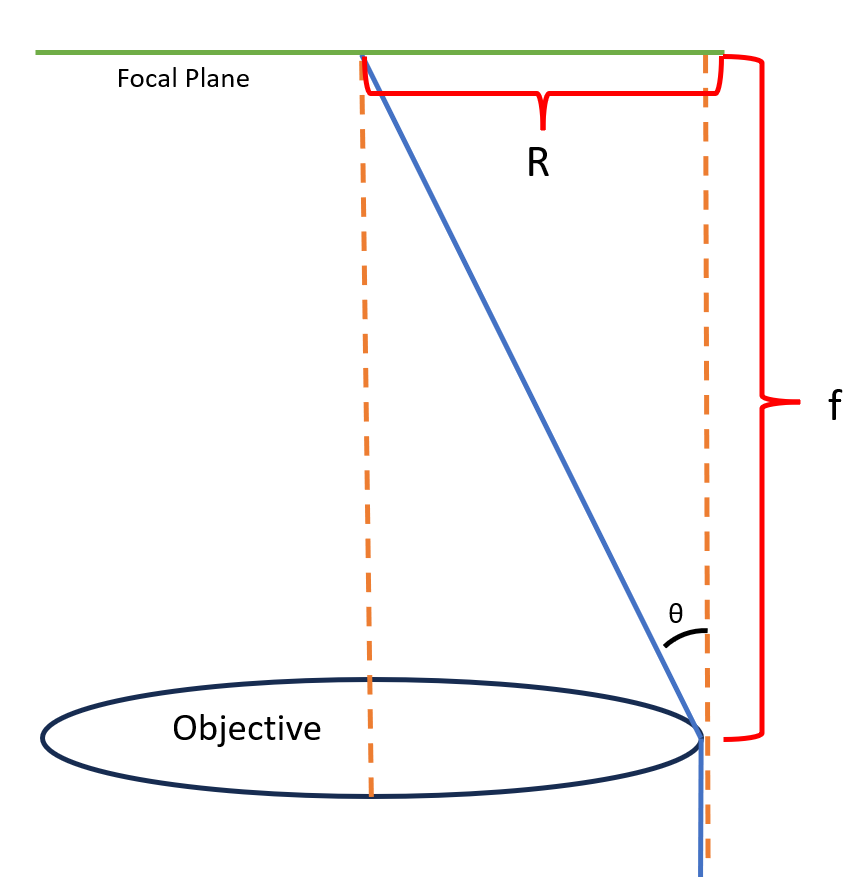
\includegraphics[width=0.3 \linewidth]{image2.png}
    \caption{Diagram of an idealized objective lens focusing to its focal plane through a single medium homogeneous medium.}
    \label{fig:enter-label}
\end{figure}
\\Note that the focal length of the lens is adjacent to the radius of its distance from the optical axis, with the angle $\theta$ being equivalent to the angle between the ray and the focal length side. Thus, trigonometrically, we see that $R / f= \tan \theta$. We can then use Taylor's expansion to approxiamte the expression for small values of $\theta$ as follows.
\begin{gather}
    \frac R f=\tan \theta= \left(\theta + \frac{\theta^3}{3} + \frac{2 \theta ^5}{15}+...\right)\\
    \frac R f \approx \theta 
\end{gather}
\textbf{Note that as a matter of convention, since the angle $\theta$ is bringing the beam "Downwards" towards the optical axis from a positive radius, $\theta$ must have a negative value. It must be added somewhat inorganically if numerical computations are going to be done to avoid the ray sailing off to infinity. As it is, $f$ vanishes below, so I've  omitted this to avoid confusion.}
We can then substitute into the system of matrices above to express the system purely in terms of $R$ and $f$, values which should be readily obtained for a given optical system.
\begin{gather}
    \begin{bmatrix}
        0 \\ \theta_2
    \end{bmatrix}
    = 
    \begin{bmatrix}
        1 & D_3\\ 0 & 1 
    \end{bmatrix}
    \begin{bmatrix}
        1 & 0\\ 0 & n_2/n_3 
    \end{bmatrix}
    \begin{bmatrix}
        1 & D_2\\ 0 & 1 
    \end{bmatrix}
    \begin{bmatrix}
        1 & 0\\ 0 & n_1/n_2 
    \end{bmatrix}
    \begin{bmatrix}
        1 & D_1\\ 0 & 1 
    \end{bmatrix}
    \begin{bmatrix}
        R \\ R/f
    \end{bmatrix}
\end{gather}
We do the matrix math as follows.
\begin{figure}[h]
    \centering
    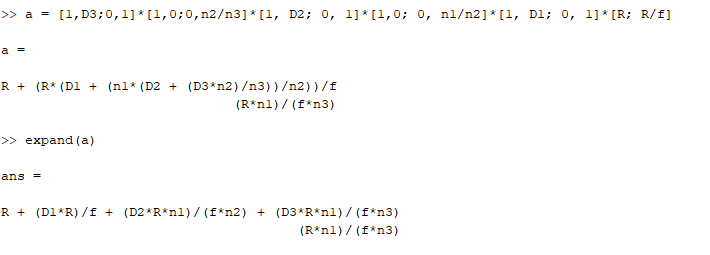
\includegraphics[width=\linewidth]{image.png}
    \caption{Matlab inputs for the matrix computation.}
    \label{fig:enter-label}
\end{figure}
\\ This leaves us with the following equation.
\begin{gather}
    0 =R + D_1 \frac R f + D_2 \frac R f \left ( \frac{n_1}{n_2} \right) + D_3 \frac R f \left( \frac{n_1}{n_3}\right)\\
    \theta_2 = \frac R f \frac {n_1}{n_3} \approx \theta \frac{n_1}{n_3}
\end{gather}
Now, we can simplify for our radial equation, moving the R over and multiplying by $\frac f R$ to simplify, giving
\begin{gather}
    -f - D_1 = \frac{n_2}{n_1}D_2 + D_3\frac{n_1}{n_3}
\end{gather}
In the case of a manipulation of the z-axis of the microscope,  everything is held constant except for $D_1$ and $D_3$, which we know is dependent on $D_1$. $D_2$ is held constant due to the static width of the glass slide. The focal length of the lens and the indicies of refraction are, of course, constants. Differentiating with respect to $D_1$, we see
\begin{gather}
    -\frac{d D_1}{d D_1} = \frac{n_2}{n_1}\frac{dD_2}{dD_1} + \frac{n_1}{n_3}\frac{dD_3}{dD_1}\\
    -1 = 0+ \frac{n_1}{n_3} \frac{dD_3}{dD_1}\\
     \Delta D_3=-\frac{n_3}{n_1} \Delta D_1 
\end{gather}
\\The notation makes the negative looks somewhat unintuitive, as though the objective and focal planes are moving in opposite directions, but this perception is a mirage caused by a misunderstanding of the variables. 
\\Interpreted correctly, this equation predicts that moving the objective further away from the sample (i.e. downwards, so that D1 increases) will bring the focal plane closer to the coverslide (i.e. downwards, so that D3 decreases), which is clearly correct. \\
Thus, the formula does predict that the focal plane and objective move in the same direction, so the math meets our intuitive expectations.


\newpage
\textbf{Pseudocode for Entire Operation}\\
\begin{enumerate}
    \item Compute timing tables and make them ready and accessible to LABVIEW
    \item Send all mirrors, etc. to start potitions
    \item Cycle
    \begin{itemize}
        \item Send pulse ot SM1 and set it to proper location.
        \item Send pulse to SM2 to align it to the propower location.
    \end{itemize}
\end{enumerate}

\newpage
\textbf{Linear Fluorescence} based on LSFM tutorial paper.\\
Density of excited flourophores per second is given by 
\begin{gather}
    N_{1p}=\delta_{1p}N_0 \frac{I_v}{h\nu}
\end{gather}
for $I_\nu$ is excitation beam intensity frequency at photonic frequency $\nu$ and the Plank constant $h$. From this we can determine the emitted number of photons per second $\Theta_{em}$ from a laser beam with cross section $S$ interacting with a fluorophore with quantum yield $\Phi$ across interaction length $l$ to give
\begin{gather}
    \Theta_{em} = \Phi \cdot N_{1p} \cdot S \cdot l.
\end{gather}
Can use Near Infared Radiation for nonlinear flourescence but I'm ignoring this.\\
We can find the beam waste of a Gaussian beam $w_0$ to a first order approximation by assuming it is equal to the axial resolution 
\begin{gather}
    R_{axial}=2w_0=2\left( \frac{f\lambda}{\pi D}\right)
\end{gather} 
for $f$ is focal length, $D$ is diameter, and $n$ is refractive index. Similarly, the field of view is euqal to the FWHM fo axial intensity distribution and is given by
\begin{gather}
    FOV=2(RaylieghRange)=2\frac{\pi w_0^2}\lambda
\end{gather}
If using an 
\newpage
\begin{center}
    Size of Incoming Light Sheet
\end{center}
The incoming light sheet needs to match the size of the back aperture of the objective in size. This means that the beam expander needs to be callibrated to match the back aperture in both dimensions without the cylindrical lens in place. The objectives we have make use of an $f=200mm$ tube lens, which works with the objective acting as the second ideal lens in a "Galilean Telescope" style setup. Note that SM1 is conjugate to the back focal plane of the objective, while SM2 is conjugate to the focal plane of the objective. Thus the size of the light sheet at the BFP is conjuigate to its size at SM1. Recall that we can relate the focal length of the tube lens and the focal length of the objective with the expression 
\begin{gather}
     \frac{f_{TL}}{magnification} = f_{obj}.
\end{gather}
Our tube lens is 200mm, so for a 60X objective we have an objective focal length of 6.66mm. \textbf{The rays make similar triangles on either side of the focal plane, which trigonometrically implies that the objective aperture should be 60X smaller than the beam at it enters the tube lens.}
So the beam should have a radius of 60X the back aperture of the objective. In general, the beam should have a radius
\begin{gather}
    R_{min-beam}=R_{obj}*\frac{1}{M}
\end{gather}
for $M$ is magnification.\\\\
OKAY THAT WAS WRONG!\\
\begin{center} \textbf{Attempt II:} \end{center}
So, we need to figure out the radius of the beam necessary to fill the back aperture of the objective. Let us proceed via matrix formalism. The beam is given by 
\begin{gather}
    \begin{bmatrix}
        R_{A} \\ \theta_2
    \end{bmatrix}
    =
    \begin{bmatrix}
        1 & D\\ 0 & 1 
    \end{bmatrix}
      \begin{bmatrix}
       R_{B} \\ \theta
    \end{bmatrix}
\end{gather}
which gives that 
\begin{gather}
    R_{A}=R_{B} + D\theta\\
    \theta_2 = \theta.
\end{gather}
We can then of course solve for $R_{BW}$:
\begin{gather}
    R_{B} = R_{A}- D\theta
\end{gather}
Note that the focal length of the TL is 200nm. As shown above, $\theta \approx \frac{R}{f}$.\textbf{ Additionally, as a matter of convention, since the angle $\theta$ is bringing the beam "Downwards" towards the optical axis from a positive radius, it must have a negative value, which we need to add somewhat inorganically, so} $\theta \approx \frac{R}{-f}$. We can then plug this in. $R$ is the radius of the beam at the lens, which of course here is $R_B$. Therefore, we have
\begin{gather}
     R_{B} = R_{A}- D\frac{R_B}{-f}\\
     R_A = R_B (1+\frac D {-f})\\
     R_B = \frac{R_A}{1-\frac D f}.
\end{gather}
This gives the result that if the beam approaches a non-zero $R_A$ at the focal plane $D=f$, the Radius will be an undefined value. $R_B$ also flips and becomes negative if $D>f$, which implies that the ray is now on the opposite side of the optical axis, as it ought to be on the other side of the focal plane. Some quick number crunching shows this to provide reasonable answers.The diameter of the filter holders is 32mm.
\newpage
\begin{center}
    \textbf{Gaussian Analysis of the Laser Beam}
\end{center}
\fbox{\begin{minipage}{\textwidth}
\textbf{Summary\\ For a Gaussian Laser beam, the power of a beam transmitted through an aperture $P_R$ is dependent on beam waist $w(z)$, the radius of the aperture $R$, and the total power of the beam $P_0$ as follows:}
\setcounter{equation}{0}
\begin{gather}
    P_R = P_0 \left[1-\exp{\left(\frac{-2R^2}{w(z)^2}\right)}\right]
\end{gather}
\end{minipage}}
\begin{center}
    \textbf{Derivation}
\end{center}
The function given above may be derived from a Gaussian function as follows. (It may also be verified by digging through the Wikipedia page on Gaussian beams. See https://en.wikipedia.org/wiki/Gaussian\_beam\\\#Power\_and\_intensity.) A generic 2D Gaussian, such as a Gaussian laser's intensity distribution, is given by 
\begin{gather}
    f(x,y) = e^{-x^2 - y^2}.
\end{gather}
More generally, it may be written as 
\begin{gather}
    f(x,y) = A \exp \left[-\left(\frac{(x-x_0)^2}{2\sigma_x^2} + \frac{(y-y_0)^2}{2\sigma^2_y} \right)\right]
\end{gather}
In the case of a laser, let us a assume that the beam is radially symmetric and centered about the origin. Then we may write:
\begin{gather}
    f(x,y) = A \exp \left[-\left(\frac{x^2+y^2}{2\sigma^2}\right)\right]
\end{gather}
Lets integrate this from negative infinity to infinity to find the total power of the laser.
\begin{gather}
    P= A \int^\infty_{-\infty} \int^\infty_{-\infty} A \exp \left[-\left(\frac{x^2+y^2}{2\sigma^2}\right)\right] dx dy\\
    P = A \int^{2\pi}_{0} \int^{\infty}_{0} \exp \left[-\left(\frac{r^2}{2\sigma^2}\right)\right] d\theta \, r dr\\
    P = 2\pi A \int^{\infty}_{0} \exp \left[-\left(\frac{r^2}{2\sigma^2}\right)\right] \, r dr
\end{gather}
More generally, we can find the power of the laser passing through an aperture of radius $R$ by integrating from 0 to $R$.
\begin{gather}
       P = 2\pi A \int^{R}_{0} \exp \left[-\left(\frac{r^2}{2\sigma^2}\right)\right] \, r dr
\end{gather}
This integral may be solved without too much fuss via complex analysis, but for the sake of convenience I use the identity given by equation 3.321.4 in \textit{A Table of Integrals, Series, and Products, 8th Edition} by Daniel Zwilliger:
\begin{gather}
    \int^b_0 r e^{-ar^2} dr = \frac{1-\exp\left(-a^2b^2\right)}{2a}.
\end{gather}
Using this identity, we see that
\begin{gather}
    P_R = 2\pi A \sigma^2 \left[ 1-\exp(-\frac{R^2}{2\sigma^2})\right]\\
    P_{full} = \lim_{x\to\infty} P_R  = 2\pi A \sigma^2 [1]
\end{gather}
In defining this, we have assumed that the intensity profile, rather than the full power, is fixed. This isn't really useful to a fixed-power laser application: we want to find percentage of set power which passes through a certain radius. We therefore substitute the expression for full power into the expression for relative power.
\begin{gather}
     P_R = P_{full} \left[ 1-\exp\left(-\frac{R^2}{2\sigma^2}\right)\right]
\end{gather}
By convention, it is useful to talk about beam waist $w$, which is a diameter rather than the standard deviation we used, which is a radial measurement. Using $w=2\sigma$, we see that
\begin{gather}
    P_R = P_{full} \left[ 1-\exp\left(-\frac{2R^2}{w^2(z)}\right)\right].
\end{gather}
$\mathcal{Q}.\mathcal{E}.\mathcal{D}.$\\
Let us assume our infinity-focused Gaussian laser beam has a Rayleigh length much longer than the optical path of our system, so that $w(z)\approx W_0$. Then we can find the beam waist of our laser to be
\begin{gather}
    1-\frac{P_R}{P_0} = \exp{\frac{-2R^2}{W_0^2}}\\
    \ln{\left( 1-\frac{P_R}{P_0}\right)}=\frac{-2R^2}{W_0^2}\\
    W_0 = \sqrt{\frac{-2R^2}{\ln{\left( 1-\frac{P_R}{P_0}\right)}}}
\end{gather}
Then plugging our real world values for HESTIA for apetures of $\diameter = 0.9mm, 3.6mm$ and power outputs $P_R/P_0 =  .24mW/2.5mW$ and $2.0mW/2.5mW$ respectively. We get $w=4.01mm$ in either case.
\newpage
\begin{center}
    \textbf{Computing the beam waist at the focal plane}
\end{center}
Recall that previously, we used two diameters and the Gaussian power transmission through an aperture to find (in both cases) what our predicted beam width is $W_0=2.00mm$. Now, given an infinity-focused beam (i.e. Rayleigh length >>1) of a given width, we should be able to compute the new beam waist at the focal plane after it has passed through a lens using the following equation (Fundamentals of Photonics, 2nd ed., 3.2-13)
\begin{gather}
    W_0'= \frac{W_0}{\sqrt{1+(z_0/f)^2}}\\
    z' = \frac{f}{1+(f/z_0)^2}
\end{gather}
Note in our case, the Rayleigh length of the Gaussian laser beam $z_0>>1$, so we can instead use 3.2-17 to see
\begin{gather}
    2W_0' \approx \frac 4 \pi \lambda F_\#\\
    2W_0' \approx \frac 4 \pi \lambda \frac f D\\
    2W_0' \approx \frac 4 \pi \lambda \frac f {\diameter_{BFP}}
\end{gather}
We can just assume that the diameter of the BFP is at least $2W_0$ to give us the approximate answer for any objective. Note we can also plug into (21) for a more precise answer.
At the focal plane of the 125mm lenses, we have
\begin{gather}
    2W_0' \approx \frac 4 \pi \lambda \frac{125mm}{2(4mm)}\\
    2W_0' \approx 20 \lambda\\
    2W_0' = 22.3 \mu m
\end{gather}
for 561nm light. This would be easy to test via implementing a pinhole and checking to see if the power percentage transferred through the aperture is consistent with (1).\\
For the 60x TIRF objective with .11mm working distance.  (I'm not sure about effective focal distance?) Alternately, we can do the Focal Length by doing $F_{TL}/M = 200mm/60 = 3.33mm$ so lets just go with 3.3mm. So we have something like this:
\begin{gather}
    2W_0' \approx \frac 4 \pi \lambda \frac{3.33mm}{2(4mm)}\\
    2W_0' \approx .297 \mu m
\end{gather}
This seems unreasonably small I think. Note that with a different formulation
\begin{gather}
    W_0' = \frac{f \lambda }{\pi W_0} = .1487\mu m
\end{gather}
so we are being consistent at least.\\
Note, however, that this is the $W_0$ which is defined as the point where the intensity of the beam has fallen to $1/e^2$ of its maximum. Lets convert to $W_{FWHM}$ to make things simpler. We know that for Gaussian Beams, $W_0=0.843218*FWHM$, so $FWHM = .176\mu m$.

Its necessary to point out that Chad claims (and I'm sure he is correct) that \textbf{Gaussian Optics does not hold for objectives}. He does some rather complicated math to attain:
\begin{gather}
    FWHM_A=4.81 \mu m\\
    FWHM_L = 771nm
\end{gather}
for a Gaussian lightsheet in the axial and lateral directions respectively.
Chat sites the following in his computations (see p41 of his thesis).
    Wolf, E., Electromagnetic Diffraction in Optical Systems .1. An Integral Representation of the Image Field. Proceedings of the Royal Society of London Series a-Mathematical and Physical Sciences, 1959. 253(1274): p. 349-357.
203. Richards, B. and E. Wolf, Electromagnetic Diffraction in Optical Systems .2. Structure of the Image Field in an Aplanatic System. Proceedings of the Royal Society of London Series a-Mathematical and Physical Sciences, 1959. 253(1274): p. 358-379.
204. Chon, H.S., et al., Dependence of transverse and longitudinal resolutions on incident Gaussian beam widths in the illumination part of optical scanning microscopy. J Opt Soc Am A Opt Image Sci Vis, 2007. 24(1): p. 60-7.


\newpage
\begin{center}
    \textbf{Finding the Correct Beam Waist}
\end{center}
Greatest objective apertures has $\diameter\approx 12mm$, but due to the magnification of the tube-relay lens system, before the tube lens is really more like $\diameter_{effective} \approx 7.5mm$. {Note I'm excluding the 10x observer, which has $\diameter_{effective} \approx 7.6mm$ but I presume won't be used enough for the slight underfilling to particularly matter.} We want to have 90\% of the light in the BFP to strike a good balance between minimizing the width of the lightsheet and not having a massive beam that sheds too much power when it enters objectives with smaller BFPs.\\
We know that the beam is Gaussian, so the beam's intensity can be modeled by an error function. So we can use $erf{x}$ to find the amount of light outside a given number of standard deviations $x$ from the center of the objective. In order to get 90 \% of the light inside, we want to have 95\% on one side of the Gaussian and 95 \% on the other. Using the inverf function in MATLAB, we find that we stay $1.38\sigma$ from the center of the beam. This implies that we need to size the beam such that $2.77 w \approx 7.5mm$, so that $\sigma \approx 2.71mm$.\\
In a sense, the objective's back aperture acts as a, well. aperture, so we can use our power transmission through a pinhole here to double check we are getting the right amount of power. We can use equation 12 above to double check that we have 90\% of the light passing as anticipated. We plug in $R^2/\sigma^2=2.77$, and see that $P_R \approx 1$. \textbf{Hmm something is off here!}\\
I think I errred by assuming that a 2D Gaussian beam follows a standard, 1D error function. If we reverse engineer equation 13 to figure out how much beam to cut out to allow 90\% of the power through, we see that $R/w \approx 1.08$ does the trick. So, according to this method, we need $7.5mm/w\approx 1.08$, which gives $w\approx 6.95mm$. A good way to callibrate the beam waist may be to set an aperture to $\diameter \approx 14mm$ so that $R \approx 7mm$, then adjust the beam width until, according to (13), 86.5\% of the power is transmitted. This should mean that $w=R = 7mm$.\\
Rich agrees with my logic that we should use the ''beam through the aperture treatment'' rather than the erf treatment, since the ERF doesn't account for two dimensionality.
\newpage
\begin{center}
    \textbf{FIOLKA Lightsheet Computations}\\
\end{center}
Note the primary source for this work is Fiolka's Lightsheet literature review. The beam waist in a LSFM system is given by 
\begin{gather}
    \omega_0 \approx \frac{0.85 \lambda}{2 NA}
\end{gather}
    Where NA is the NA of the illumination objective and $\lambda$ is the excitation wavelength. The lateral beam radius is given by 
    \begin{gather}
        \omega(x) = \omega_0 \sqrt{1 + \left(\frac{x}{x_R}\right)^2}\\
        x_R = \frac{n \pi \omega_0^2}{\lambda}
    \end{gather}
    where $x_R$ is the Rayleigh length in the lateral direction.
    In the y-direction, the beam is essentially of infinite width and thus limitless depth of focus, as this is the broad side of the sheet. The only limitation here is the optical train componenets.\\
    The lateral resolution of LSFM (i.e. in the x-y plane direction) is defined by 
    \begin{gather}
        \Delta r = \frac{\lambda_{em}}{2 NA_{det}}
    \end{gather}
    for the emission and detection wavelengths. This is because this is the FWHM radius of the beam, which is the point at which two airy disks would reach thier first trough and be distinguishable.\\
    The axial resolution is given by the product of the illumination and detection point spread function, which in turn depend on the excitation and emission wavelengths adn the NA of the objective (which in our case is combined). In general, thinner light-sheets are generated by higher NA objectives with higher axial resoltuion but also have narrower Rayleigh lenghts and thus worse field of view. In other words, it is messy, but can be approximated (assuming $NA_{exc}=NA_{ill}$) by
    \begin{gather}
        \Delta z \approx \left( \frac{2 NA_{ill}}{\lambda_exc} + \frac{n (1-\cos \theta)}{\lambda_em}\right)^{-1}
    \end{gather}
    where $\theta$ is the half-angle of the detection objective
    \begin{gather}
        \theta = \arcsin\left(\frac{NA}{n}\right)
    \end{gather}
    Now, we must compute the ideal beam width and compare this with our own findings. For our TIRF objective, which has an NA of and 561nm laser light,
    \begin{gather}
        \omega_0 \approx \frac{0.85\cdot561nm}{2*(1.5)}\\
        \omega_0 \approx 158.95nm
    \end{gather}
We can also use a beam simulator to verify our result--see https://github.com/remachae/beamsimulator. We end up with a main lobe width of .32$\mu m$, which is equivalent to $\omega_0=160nm$; our answer checks out.

\newpage
\begin{center}
    \textbf{Works Cited}\\
    Insert later. Include optics book, HIST paper, HIST guide paper, microscopy book, etc.
\end{center}
\begin{center}
    Links to helpful webpages used in these calculations
\end{center}
https://www.microscopyu.com/tutorials/spatial-resolution-in-digital-imaging\\
Optics In Motion User Manual for User’s Manual for OIM100 series FSM Models OIM101, OIM102, OIM102.3\\
New HIST Camera manual etc available at: https://andor.oxinst.com/products/scmos-camera-series/zyla-4-2-scmos